\documentclass[14pt, fleqn, xcolor={dvipsnames, table}]{beamer}
\usepackage[T2A]{fontenc}
\usepackage[utf8]{inputenc}
\usepackage[english,russian]{babel}
\usepackage{amssymb,amsfonts,amsmath,mathtext}
\usepackage{cite,enumerate,float,indentfirst}
\usepackage{cancel}

\usepackage{tikz}                   
\usetikzlibrary{shadows}

% \usepackage{enumitem}
% \setitemize{label=\usebeamerfont*{itemize item}%
%   \usebeamercolor[fg]{itemize item}
%   \usebeamertemplate{itemize item}}

\graphicspath{{images/}}

\usetheme{Madrid}
\usecolortheme{seahorse}
\renewcommand{\CancelColor}{\color{red}}

\setbeamercolor{footline}{fg=Blue!50}
\setbeamertemplate{footline}{
  \leavevmode%
  \hbox{%
  \begin{beamercolorbox}[wd=.333333\paperwidth,ht=2.25ex,dp=1ex,center]{}%
    И. Кураленок, Н. Поваров, Яндекс
  \end{beamercolorbox}%
  \begin{beamercolorbox}[wd=.333333\paperwidth,ht=2.25ex,dp=1ex,center]{}%
    Санкт-Петербург, 2013
  \end{beamercolorbox}%
  \begin{beamercolorbox}[wd=.333333\paperwidth,ht=2.25ex,dp=1ex,right]{}%
  Стр. \insertframenumber{} из \inserttotalframenumber \hspace*{2ex}
  \end{beamercolorbox}}%
  \vskip0pt%
}
\newcommand\indentdisplays[1]{%
     \everydisplay{\addtolength\displayindent{#1}%
     \addtolength\displaywidth{-#1}}}
\newcommand{\itemi}{\item[\checkmark]}

\title{Линейные модели: уменьшаем variance\\\small{}}
\author[]{\small{%
И.~Куралёнок,
Н.~Поваров}}
\date{}

\begin{document}

\begin{frame}
\maketitle
\small
\begin{center}
\vspace{-60pt}
\normalsize {\color{red}Я}ндекс \\
\vspace{80pt}
\footnotesize СПб, 2013
\end{center}
\end{frame}

\section{Variance линейных моделей слишком велик!}
\begin{frame}{Переобозначение параметра решающей функции!}
$\lambda$ --- мало. С сегодняшнего дня вместо него $\beta$
$$
F(x, \lambda) \to F(x, \beta)
$$
Слайды предыдущих лекций переделаем.
\end{frame}

\begin{frame}{Воспоминания о былом}
\begin{itemize}
  \item Из второй лекции мы знаем, что линейные модели имеют большой разброс решений
  \item Из 7-й лекции мы знаем, что меньше разброс нам не сделать с избранной целевой функцией (теорема Гаусса-Маркова)
\end{itemize}
$\Rightarrow$ будем менять целевую функцию: вводить условия, или менять саму $T$.
\end{frame}

\subsection{Пример с очередным Сифоном/Бородой}
\section{Поиск условного оптимума}
\begin{frame}{Хорошие решения}
\begin{enumerate}
  \item Предположим, что данные $y$ y нас шумные
  \item Введем чувство прекрасного $-R(\beta)$ 
\end{enumerate}
Тогда нашу проблему можно свести к:
$$\begin{array}{l}
\arg \min_\beta R(\beta) \\
\| X\beta - y\| < \epsilon
\end{array}$$
Ну или так:
$$\begin{array}{l}
\arg \min_\beta \| X\beta - y\| \\
R(\beta) < p
\end{array}$$
\end{frame}

\begin{frame}{Преобразование целевой функции}
$$
\arg \min_\beta \| X\beta - y\| + \lambda R(\beta)
$$
Можно найти такой параметр $\lambda$, который будет давать решение задачи на предыдущем слайде. В смысле оптимизации проблемы эквивалентны.
\end{frame}


\begin{frame}{C байесовой точки зрения}
Строго говоря, мы ввели prior на распределение решений:
$$\begin{array}{l}
\arg \max_\beta P(y|X\beta) P(\beta) \\
= \arg \max_\beta \sum_i log P(y_i|x_i\beta) + log P(\beta)
\end{array}$$
Если предположить нормальность $P(y_i|x_i\beta)$, то проблема становится очень похожей на то, что мы уже видели:
$$
= \arg \min_\beta \|X \beta - y\| - z log P(\beta)
$$
где $z$ --- ошметки нормальности.
\end{frame}

\begin{frame}{Виды prior}
Какими бывают $-log P(\beta)$:
\begin{description}
  \item[$\|\beta\|_0$] --- бритва Оккама, MDL, etc.;
  \item[$\|\Gamma\beta\|_2$] --- нормальное распределение c $\Sigma = \Gamma^{-1}$ и $\mu = 0$;
  \item[$\|\beta\|_1$] --- распределение Лапласа;
\end{description}
Как можно видеть все это добро обобщается в $l_q$.
\end{frame}

\begin{frame}{Сравнение prior'ов в случае $l_1$ и $l_2$}
\begin{center}
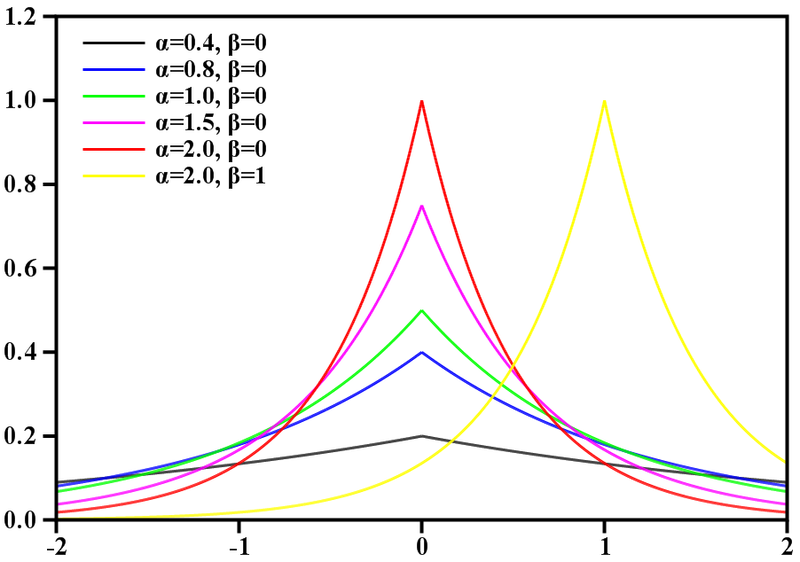
\includegraphics[width=0.4\textwidth,height=0.5\textheight]{800px-Laplace_distribution.png} 
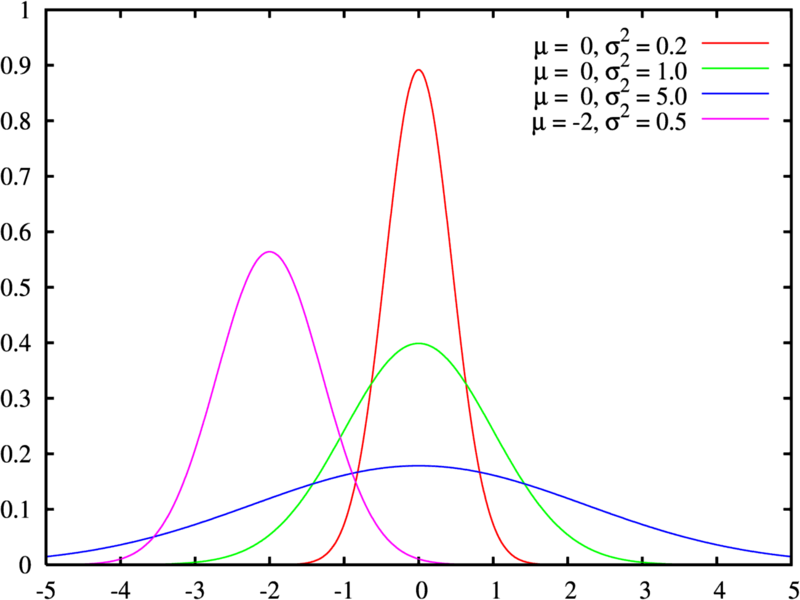
\includegraphics[width=0.4\textwidth,height=0.5\textheight]{800px-Normal_distribution.png} 
\end{center}
Картинки из википедии
\end{frame}

\subsection{Почему все это очень клево ложится на ML}
\begin{frame}{Как это относится к ML}
Точное решение в $L$ несет слишком много информации о обучающей выборке, поэтому точно оптимизировать смысла нету. Таким образом условие:
$$\begin{array}{l}
\max R(\beta) \\
\|X\beta - y\| < \epsilon
\end{array}$$
хорошо ложится на ML. При этом возможность выбора $R$ позволяет рассказать наши ожидания от структуры решения.
\end{frame}

\begin{frame}{Как это называется}
\begin{description}
  \item[$\|\beta\|_0$] --- Best Subset;
  \item[$\|\Gamma\beta\|_2$] --- регуляризация Тихонова/ridge regression;
  \item[$\|\beta\|_1$] --- least absolute shrinkage and selection operator (LASSO);
\end{description}
Также рассматривается обощение на $l_q$.
\end{frame}

\subsection{Картинки разных условий}

\begin{frame}{Геометрия LASSO}
$$\begin{array}{l}
\min_\beta {\color{blue} \|X\beta - y\|} \\
{\color{red} \|\beta\|_1 < p}
\end{array}$$
\begin{center}
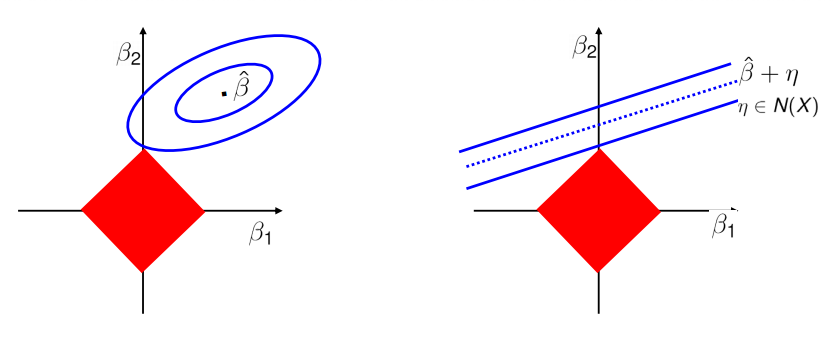
\includegraphics[width=0.9\textwidth]{Geometric_View.png} 
\end{center}
\footnotesize
Картинки из ICML 2010 Tutorial (Irina Rish, Genady Grabarnik)
\end{frame}

\begin{frame}{Геометрия LASSO II}
\small
Рассмотрим зависимость компоненты решения $\beta_0$ от решения безусловной системы $\hat{\beta} = \left(X^TX\right)^{-1}X^Ty$.
\begin{center}
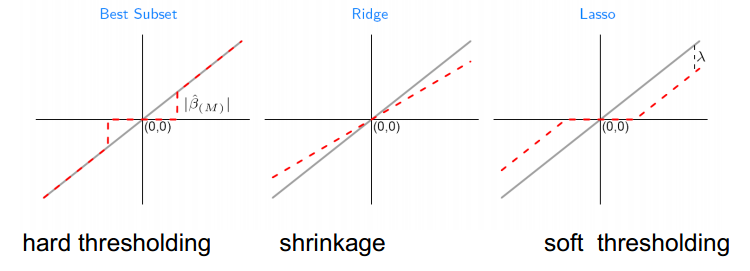
\includegraphics[width=0.9\textwidth]{shrinkage.png} 
\end{center}
\footnotesize
Картинки из The Elements of Statistical Learning (Hastie, Friedman and Tibshirani, 2009)
\end{frame}

\section{Как считать}
\begin{frame}{Пара слов об оптимизации $l_0$}
\small
$l_0$ --- естественное условие на решение: ``меньше фишек --- легче думать'' \\
Точное решение однако найти очень дорого: проблема $NP$-сложная. Поэтому есть масса работ по тому как найти приближенное решение:
\begin{itemize}
  \item Если $n < 40$ есть работа ``Regressions by Leaps and Bounds'' (Furnival and Wilson 1974) + CV для выбора эффективного ограничения
  \item Взад-назад селекшен (Forward/Backward-Stepwise Selection): выбрасываем или добавляем фичу с наибольшим/наименьшим Z-score
  \item Приближение с маленьким $q$
  \item ``Хитрые'' переборы многомерного креста
\end{itemize}
\end{frame}

\begin{frame}{Оптимизация $l_1$ и $l_2$}
\small
В случае ridge regression все просто:
$$
\beta_0 = \left(X^{T}X+ \Gamma^{T} \Gamma\right)^{-1}X^{T}y
$$
А в случае LASSO все не так просто, так как $T$ негладкая. Поэтому там почти градиентный спускъ. Есть несколько способов:
\begin{itemize}
\small
  \item Оригинальный пошаговый
  \item LARS
  \item Покоординатный спуск (посмотреть дома)
  \item ISTA
  \item FISTA
  \item etc.
\end{itemize}
\end{frame}

\subsection{Stagewise LASSO}
\begin{frame}{Оптимизация $l_1$ и $l_2$}
\begin{itemize}
\small
  \item Оригинальный пошаговый
  \item LARS
  \item Покоординатный спуск (посмотреть дома)
  \item ISTA
  \item FISTA
  \item etc.
\end{itemize}
\end{frame}

\subsection{LARS}
\subsection{ISTA}
\subsection{Как LASSO работает на Сифоне-Бороде}
\section{ElasticNet vs $l_{0.5}$ vs. $l_{1.1}$}
\subsection{Объем данных vs $q$}
\section{Регуляризация}
\section{Домашнее задание}

\end{document}
